\section{Inlet Design}

\subsection{Design Overview - John Ellis}
\subsubsection{Requirements}
Requirements stated that the inlet would be a chin-type inlet, which would reserve the nose of the vehicle for installation of sensors. The chin-type inlet precluded the use of the more common, and more analytically analyzable, axisymmetric spike inlet, as seen on the operational BrahMos missile system in Fig. \ref{fig:BrahMos}. 
\begin{figure}[H]
\centering
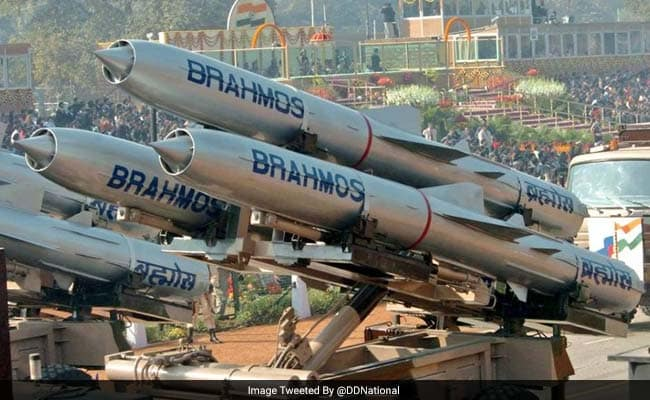
\includegraphics[width=.5\textwidth] {JWE_Figures/BrahMos_Intake2.jpg}
\caption{Axisymmetric intake as seen on the Indian/Russian ramjet missile, BrahMos \cite{varma_2018}}
\label{fig:BrahMos}
\end{figure}

Additional inlet performance requirements could be derived from the conceptual development of other subsystems and the mission envelope. These include:
\begin{enumerate}
\item The inlet shall provide air mass flow of 2 kg/s air flow at cruise.
\item The inlet shall be designed to operate at Mach 2.5 at cruise.
\item The inlet shall be designed to operate in an ideal Mach range of 2.25 to 2.5 during the SFRJ burn.
\item The inlet shall maximize pressure recovery while minimizing shock pattern complexity.
\end{enumerate}


\subsubsection{Physical Design}
 While data on current designs is extremely limited due to the confidential nature of high-speed military propulsion, there was a small pool of academic and old military research to pull from. The Advanced Strategic Air-Launched Missile (ASALM, seen in Fig. \ref{fig:ASALM}) was greatly influential in the design of the SFRJ intake and inlet integration. The ASALM was a weapons development platform investigated during the late 1970s. It was designed to be an air-to-ground missile with nuclear capability and to cruise at around Mach 4.5. Most importantly, it was an integral rocket-ramjet system designed with a chin type inlet.
 
\begin{figure}[H]
\centering
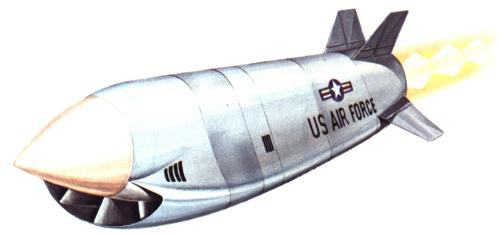
\includegraphics[width=.5\textwidth]{JWE_Figures/asalm.jpg}
\caption{Artist's rendition of what could have been the final vehicle configuration of the ASALM system. \cite{parsch}}
\label{fig:ASALM}
\end{figure}
 
The precursor to what would have been the full ASALM system was the Propulsion Technology Validation (PTV) vehicle that was used to test the design methodology and verify simulations. Seven flight tests were conducted with the PTV vehicle prior to the programs cancellation \cite{parsch}. Data relating to wind tunnel testing of the PTV vehicle was used in the basis of the SFRJ inlet design. The PTV used a two external shock system to compress the incoming air in a non-symmetric fashion. Bleed was incorporated upstream of the ramp in order to minimize boundary layer effects on the shock angles. As this was a physical system, several non-optimal geometric changes were added to aid the ability to manufacture (rounded corners, support plates, etc). A representative overview can be seen in Fig. \ref{fig:ASALM_Intern}.

\begin{figure}[H]
\centering
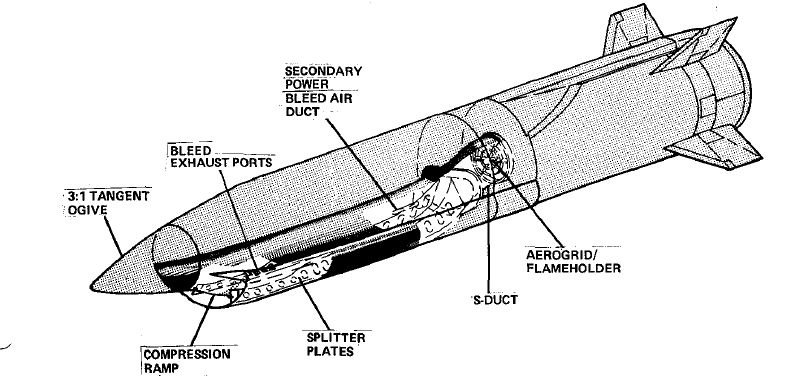
\includegraphics[width=0.9\textwidth]{JWE_Figures/ASALM_Internal.jpg}
\caption{Propulsion Technology Validation vehicle  \cite{webster_bucy_1979}}
\label{fig:ASALM_Intern}
\end{figure}

The inlet design for the SFRJ vehicle (as seen in Fig. \ref{fig:InletGeom} below) is based on the PTV design, but altered for the requirements of a different mission. While the PTV was designed for around Mach 4.5, the goal for the SFRJ is Mach 2.5. This causes the shock angle off of the nose cone to be much steeper, moving the shock away from the body and altering the cowl placement. As such, the SFRJ cowl is much further forward to minimize the distance away from the main body. Secondly, the PTV was deigned as a nuclear cruise missile against ground targets and thus needed guidance but not sensors/trackers. The nosecone for the PTV was not blunted more than was necessary for manufacturing to decrease the strength and size of the detached shock wave. The SFRJ concept is for eventual air targeting functionality and as such will need to incorporate some seeker (infrared, radar, visual, etc.). The nose cone used for the design here has a much larger blunted nose to house a seeker window, as seen on current missile systems like the AIM-9 Sidewinder. The large spherical dome also increases the lead shock angle, meaning the cowl must be even further forward for shock attachment.

The base nose cone profile is that of the Von K\'arm\'an Haak series. The Von K\'arm\'an profile was selected as previous work has shown that it develops the least amount of drag out of the common designs in high Mach flows \cite{crowell}. However, the SFRJ design has been blunted, and further analysis is needed to verify that the design is still optimal for high Mach drag reduction. The Length-over-Diameter of the nose was set to the 3:1 ratio as seen on the PTV. This ratio could benefit from further optimization for the lower Mach seen by the SFRJ, as a higher ratio would likely result in a shallower shock angle and reduce the needed forward tilt of the cowl. 

The secondary ramp on the SFRJ is set at 15\textdegree\ (measured from the direction parallel to the flow at the start of the ramp), as this was found to result in a Mach number of sub-1.4 at the inlet plane. J. Seddon \cite{seddon_goldsmith_1999} suggests that the pre-terminal shock Mach should be below 1.5 as the pressure recovery across a normal shock stronger than 1.5 results in a rapid decrease in pressure recovery. Only two shocks were  needed as the external Mach number was relatively low and this kept the complexity of the shock wave pattern down. Data from J. Seddon suggests that the increase in complexity to a three shock system would result in less than a 5\% increase in pressure recovery. Seeing as the pressure recovery was already well above 80\%, the increased complexity and 3-D flow effects was deemed to be more detrimental than beneficial.

After the terminal shock at the inlet plane, the flow is passed through a constant area, semi-annular duct in order to isolate any oblique shock wave trains that develop due to off-design flight and viscous effects. The length of the duct was designed according to an empirical procedure detailed by J. Mahoney \cite{mahoney_1991}. From the semi-annular duct the flow is diffused into a larger circular duct That is centered within the body of the vehicle in order to connect to the combustion chamber. This subsonic diffuser will need to be verified via CFD or wind tunnel testing as it is unclear at this point how quickly the area of the duct can expand before separation occurs. Also incorporated, but not analyzed, are flush bleed ports upstream of the second ramp.These ports are connected to an internal plenum that then dumps the bleed flow overboard, reducing viscous effects on the ramp functionality. Data compiled by J. Mahoney suggests that bleed flow rate of between 4 and 8\% results in actual pressure recoveries approximately equal to the calculated ideal recovery. Sizing and number of these flush bleed holes needs to be calculated in order to properly realize this flow rate.

\begin{figure}[H]
\centering
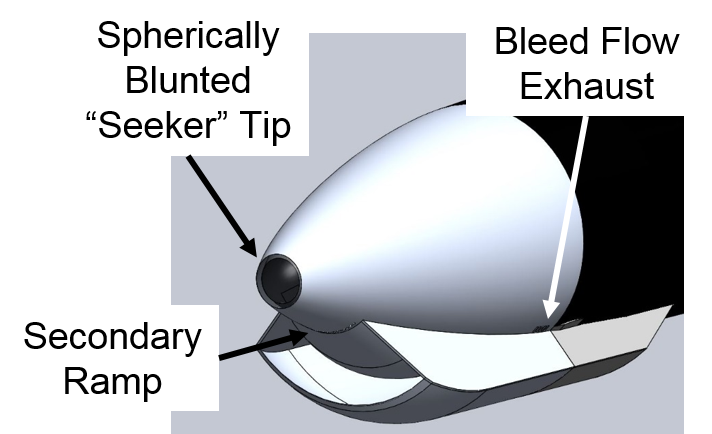
\includegraphics[width=.65\textwidth]{JWE_Figures/Nose_CAD_Iso.png}
\caption{SFRJ inlet design.}
\label{fig:InletGeom}
\end{figure}

\subsection{CFD Analysis - John Ellis}
Requiring a chin design over an axisymmetric inlet meant that a number of analytically design methods were no longer valid. Also complicating matters was the blunted nose cone, which would result in a detached shock wave. Instead of analytically methods, a computational fluid dynamics (CFD) model was needed in order to predict the flight characteristics of the inlet and alter the geometry accordingly in order to optimize for the range of the vehicle. Due to the limited knowledge of CFD at the time, many models and variations were tried, but with little success. (These can be found in Appendix A.) One model was successfully run that solved the basic shock wave pattern and produced a simplified cane curve of the air flow and pressure recovery.

For this (and all other models attempted) the inlet was simplified to an axisymmetric form that then could be used to extrapolate the performance of a chin inlet. Figure \ref{fig:InletCFDGeom} shows the surface used in the solution. Neither cowl or subsonic diffuser was modelled, as these caused issues in previous attempts at the solution. Instead, the intake plane, where a normal shock would develop at the critical, on-design condition, was demarcated to allow for easy data extraction.

\begin{figure}[H]
\centering
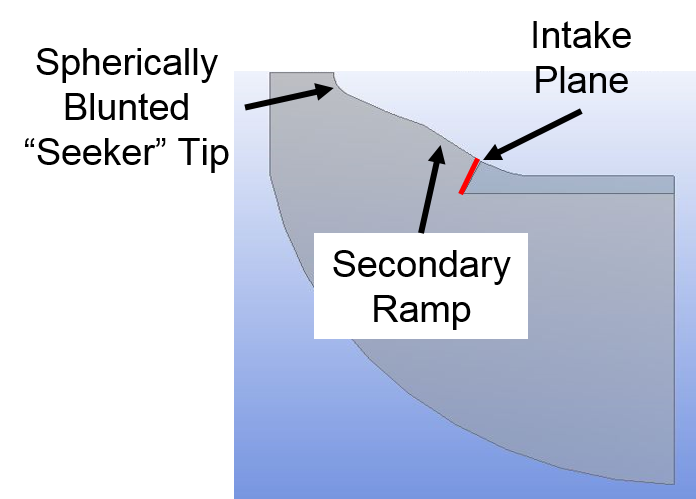
\includegraphics[width=.65\textwidth]{JWE_Figures/Nose_CFD_Surf.png}
\caption{SFRJ inlet CFD 2D surface geometry}
\label{fig:InletCFDGeom}
\end{figure}

The combination of boundary conditions as seen in Fig. \ref{fig:InletCFDBC} were used to model the nose flying at Mach numbers ranging from 1.9 to 2.7 in 0.1 Mach increments. (To simulate low and high speed flights). The model was meshed with a high density structured mesh using 894033 elements. The mesh base-size was 1e-4 m, and refined to 9e-5 m near the cowl point in order to accurately model the coalescence. An implicit density based solver was implemented, as is suggested for supersonic flow. A Courant number of 5 was used to stabilize the solution process, as higher numbers were found to cause divergence issues. 

\begin{figure}[H]
\centering
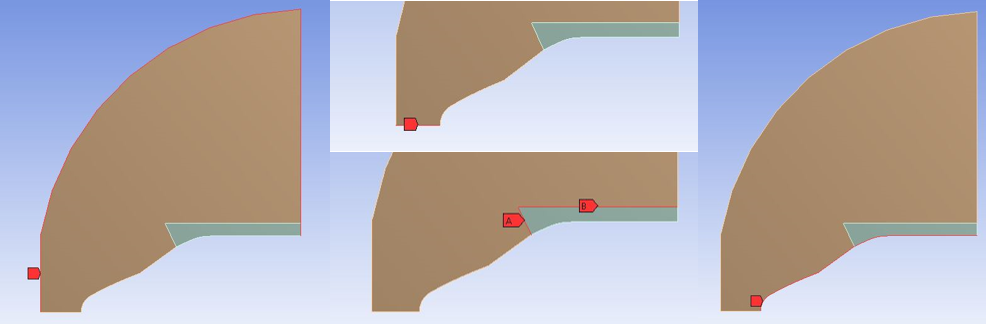
\includegraphics[width=0.98\textwidth]{JWE_Figures/CFD_BC_Group.png}
\caption{SFRJ inlet CFD boundary conditions marked in red lines. Left: Far-Field Pressure. Middle-Top: Revolution Axis. Middle-Bottom: Interior. Right: Wall}
\label{fig:InletCFDBC}
\end{figure}


The resulting flow fields were used in order to size the ramp and shift its position such that the two shock waves coalesced at the point where the cowl would sit. This was visualized by leaving the smaller portion of the surface out of the contour surface plots. Figure \ref{fig:InletCFDCon} shows both the single surface contour as well as the combine surface contour of the final design at the on-design condition of Mach 2.5.

\begin{figure}[H]
\centering
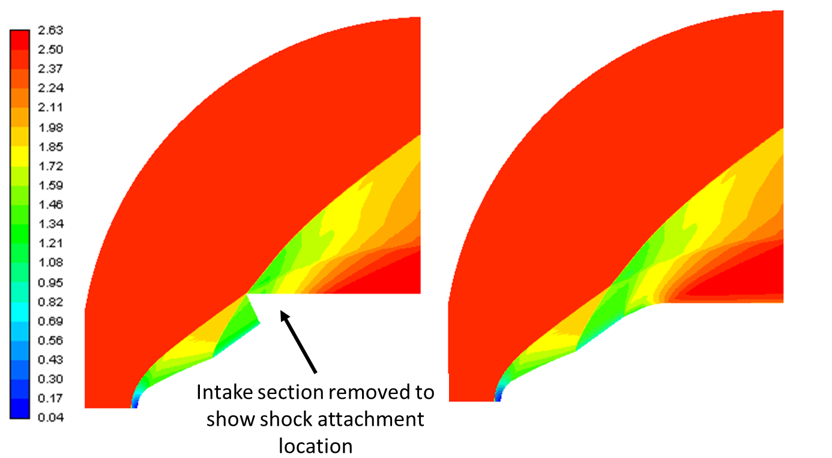
\includegraphics[width=0.75\textwidth]{JWE_Figures/CFD_Contour.png}
\caption{Mach number contour plot of the final nose cone configuration at free stream Mach of 2.5. Left: Intake section removed. Right: Combined surfaces}
\label{fig:InletCFDCon}
\end{figure}

\subsection{Simulator Integration}
\subsubsection{Mass Flow vs Back Pressure - John Ellis}
The flow properties at the intake plane were then extracted to Matlab$\copyright$ to continue the analysis procedure. At this point, normal shock equation were used to calculate the static and stagnation pressure and temperature, density, velocity, and mass flow rate. This was deemed the critical condition operating point, and was the highest mass flow that the inlet could take in at that Mach number. Recovery pressures lower than this would mean the normal shock wave is swallowed, and a stronger normal shock develops within the subsonic diffuser, but still the same amount of air is taken it. Pressures higher than this were approximated with a linear fit to an "unstart" state, or when mass is ejected from the inlet. This sub-critical state is by far the least defined, and needs further examination. However, comparing to wind tunnel tests of other chin inlets done by Hermann \cite{herrmann_2008}, it appears to be a decent first order approximation. Their wind tunnel data was compiled for this study for each Mach number into cane curves (Fig. \ref{fig:InletCane} ) that could be used in the simulation of the vehicle. The simulator would use the current time step chamber stagnation pressure as well as the free stream Mach number to see how much air mass flow the inlet would provide in a fully axisymmetric configuration. Then, using the initial simulation input of the inlet "sweep angle," scale that mass flow as a fraction over 360. (This allowed the simulator to use "sweep angle" as a variable in parameters sweep to see what mass flow would maximize the range of the vehicle.)

\begin{figure}[H]
\centering
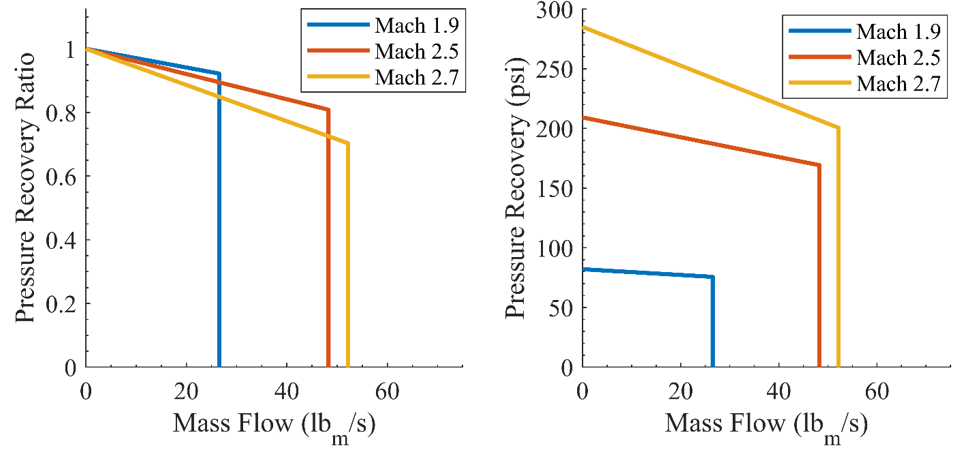
\includegraphics[width=0.95\textwidth]{JWE_Figures/CaneCurves.png}
\caption{Cane curves at the low, high, and on-design Mach numbers simulated both in recovery ratio and absolute pressure recovery}
\label{fig:InletCane}
\end{figure}

\subsubsection{Angle of Attack Adjustments - Melanie Grande}
The final piece of the simulator integration with the inlet design was to model flow and losses at various angles of attack (AoA). The effects of AoA are complex at different flight Mach numbers and with different inlet designs. Fortunately, a wind tunnel experiment by Herrmann, Triesch, and G\"ulhan of the German Aerospace Center revealed critical data points for mass flow losses and pressure recovery across chin-type inlets at various AoA and inlet sweep angles, precisely what was needed for this SFRJ concept \cite{herrmann_2008}. The experimental data for mass flow losses has been extrapolated in the SFRJ simulator, pulling the vehicle's AoA at that time step and interpolating to find the effect. The interpolated value from the reference data was also normalized to the experimental mass flow loss ratio at zero AoA, considering the differences in the reference design and the wind tunnel experiment being flown at Mach 3. The adjustments for pressure recovery at various AoA have been integrated in a different way, based on limitations with modeling the diffuser and incorporating the inlet CFD data. This is described in the previous section. 

Additionally, the SFRJ concept explored the use of "droop", an angle designed into the inlet at an offset from the main body axis. The purpose of the offset angle was to minimize losses when the average cruise AoA is known from the simulator. This simple adjustment created an "effective" AoA and air influx for the inlet. However, with the evolution of the SFRJ design, including improvements to the inlet, fin mechanisms, and lift analysis, the impact of the offset angle was considered small, as will be discussed in the Trade Studies section of this report. The final baseline design included zero offset angle.
